%!TEX program = xelatex

% ==== Part1: 引入latex需要的package,支持不同的需求,如中文、图片 ====
\documentclass[a4paper, 12pt]{article}
% \documentclass[a4paper]{report}
\usepackage[UTF8]{ctex} % 中文latex支持
\usepackage{graphicx} % 引入图片时需要的包
\usepackage{float}    % 插入图片的时候支持`H`这个位置选项
\usepackage{subcaption} % 插入多张图片到一个figure域中
\usepackage{hyperref}   % 插入超链接、TOC支持链接
\usepackage{amsmath,bm} % 一些数序符号、字符
\usepackage{listings}   % 插入代码块
\usepackage{geometry}   % 设置页面四周的边距
\usepackage{booktabs}   % 插入三线表
\usepackage{setspace}
% ==== 对引入的package配置 ====
\graphicspath{{images/}} % 配置graphicx这个包:指定图片存储的地方
\hypersetup{
  colorlinks=true,
  linkcolor=black,
  urlcolor=black,
}
% \hypersetup{ % 设置超链接和url的显示样式
%     colorlinks=true,
%     linkcolor=blue,
%     filecolor=magenta,      
%     urlcolor=cyan,
%     pdftitle={Overleaf Example},
%     pdfpagemode=FullScreen,
%     }
% \urlstyle{same}

% ==== Part2: latex文档格式配置 ====
\newif\ifchinese % 定义一个条件变量: ifchinese, 作为控制条件编译的开关
\chinesetrue % 条件编译的控制开关,注释掉此部分内容,则对应部分不会被现实
\geometry{a4paper,left=3cm,right=3cm} % 设置左右的页边距


% ==== Part3: latex文档标题部分 ====
\title{LaTex文档模版}
\author{付杰}
% \author{付杰\thanks{谢谢overleaf提供的LaTex教程}}
\date{\today}


% ==== Part4: latex文档正文部分 ====
\begin{document}
% \maketitle
% \thispagestyle{empty} % don't use footprint
% \clearpage

\pagenumbering{Roman}
\tableofcontents % 插入目录
\clearpage


% \section{条件编译:根据配置的信息,选择编译某一部分的内容}

% \ifchinese
% 这部分是条件编译的内容,必须在\textbf{chinesetrue}判定为真的时候,才会被输出
% \fi


\pagenumbering{arabic}
\setcounter{page}{1}
\section{研究背景}%
5G通信相较于4G通信,具有更高的数据速率、更低的延迟、更大的容量跟连接密度等优点。5G通信的时隙小于10ms,5G基带芯片需要在有限的计算时间内完成复杂的计算,如信号处理和调制解调、FFT计算等,这些计算为了保证时效性被硬化成了对应的加速器以保证对应的计算任务可以在规定的时隙内完成\cite{8920308}。

5G基带芯片通过引入硬件加速器来满足时间严苛的计算需求,但又因此引入了加速器的调度配置问题。
基带芯片内部有数十个硬件减速器来处理不同的复杂计算任务,
各个加速器需要被正确地配置才能工作、
各个加速器完成计算任务之后会发送中断信号给微控制器,微控制器需要及时处理器加速器的中断,才能保证5G通信的实施性\cite{9048785}。

5G设备需要在更高的频谱和更大的数据速率下运行,这可能导致设备的能源消耗增加;
而且搭载基带芯片的设备可能会采用电池进行供电,因此基带芯片内部的微控制器设计的时候需要考虑低功耗设计、并且支持在低负载的情况下进入睡眠模式\cite{9336351}。

本研究课题主要的内容是设计一款低功耗微控制器对5G基带芯片内部的加速器进行调度,
要求微控制器本身的计算性能满足加速器调度的需求、并且满足低功耗的特性;在此基础上该微处理器需要针对
微控制器需要对数十个加速器调度的应用场景做专门的优化。MCU在基带芯片中的位置如图\ref{fig:pic1}粉色虚线框部分所示。
\begin{figure}[htbp]
  \centering
  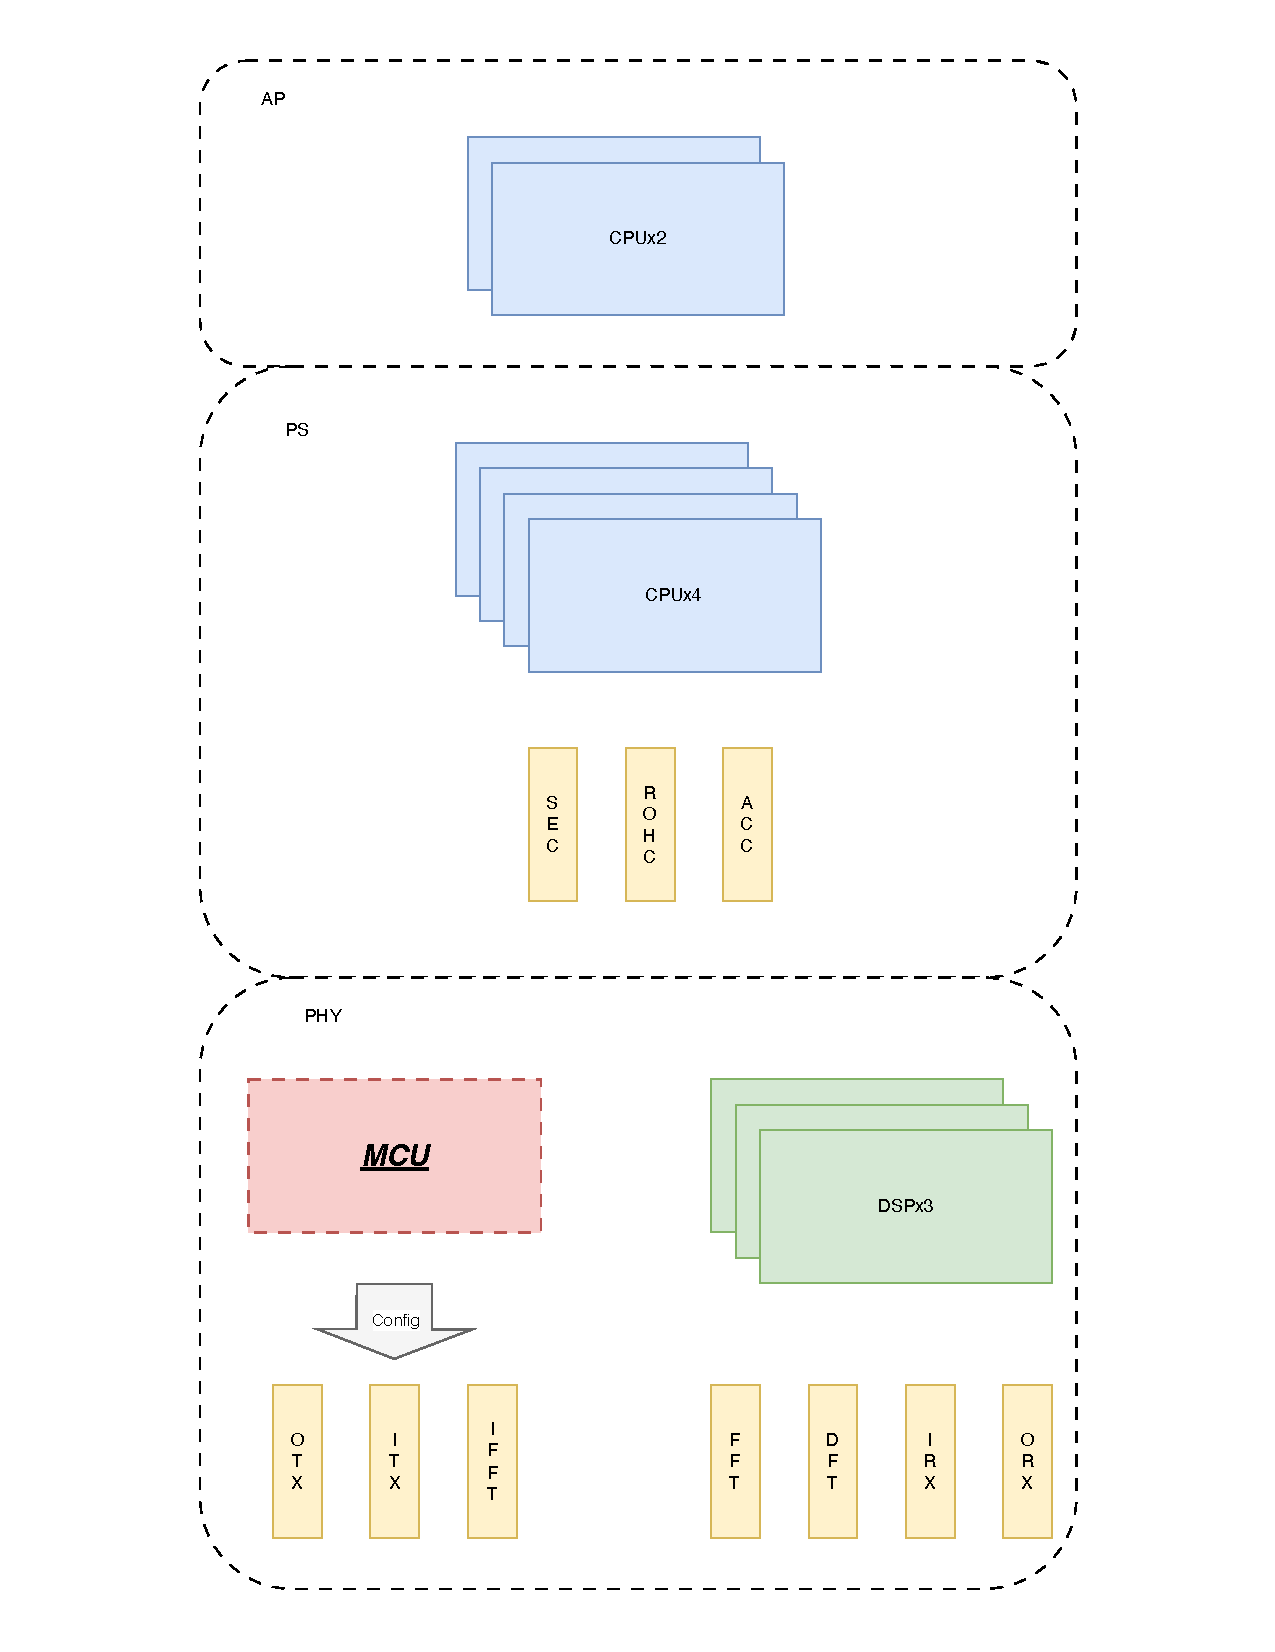
\includegraphics[scale=0.5]{./images/mcu_location.pdf}
  \caption{所设计微控制器在5G基带芯片中的位置}
  \label{fig:pic1}
\end{figure}

\clearpage
\section{研究内容及当前进度}%
本课题主要目标是基于RISC-V指令集开发MCU,用于控制5G基带芯片内部的加速器\cite{9319703}。
需要满足快速响应及低功耗的特征。本课题的研究内容主要有三个方面,如图\ref{fig:research_topics}所示。
\begin{figure}[htbp]
  \centering
  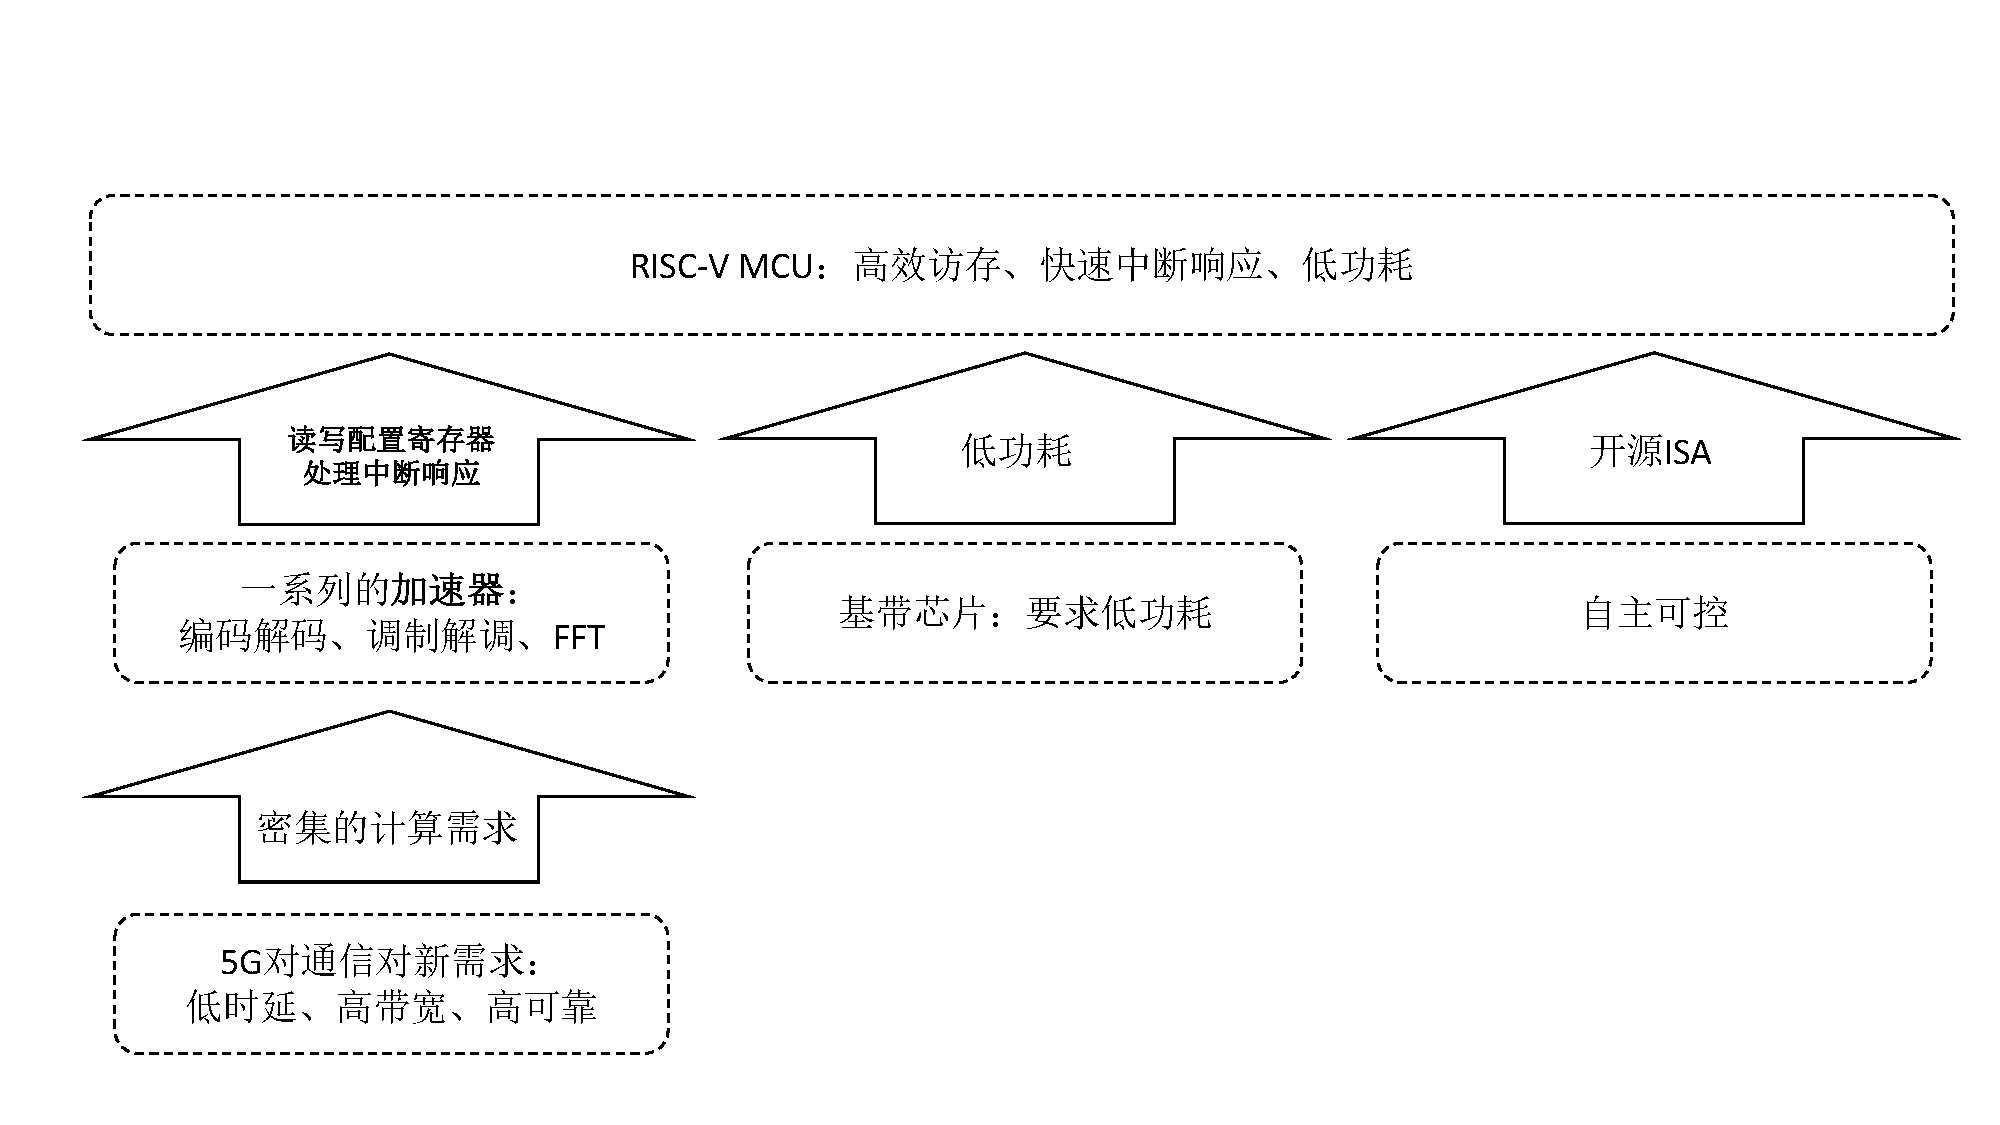
\includegraphics[width=0.8\linewidth]{./images/research_topics.pdf}
  \caption{本课题研究内容}
  \label{fig:research_topics}
\end{figure}

目前本课题主要研究内容及进度如图\ref{fig:study_progress}所示;% TBD change pic to table

\begin{figure*}[htbp]
  \centering
  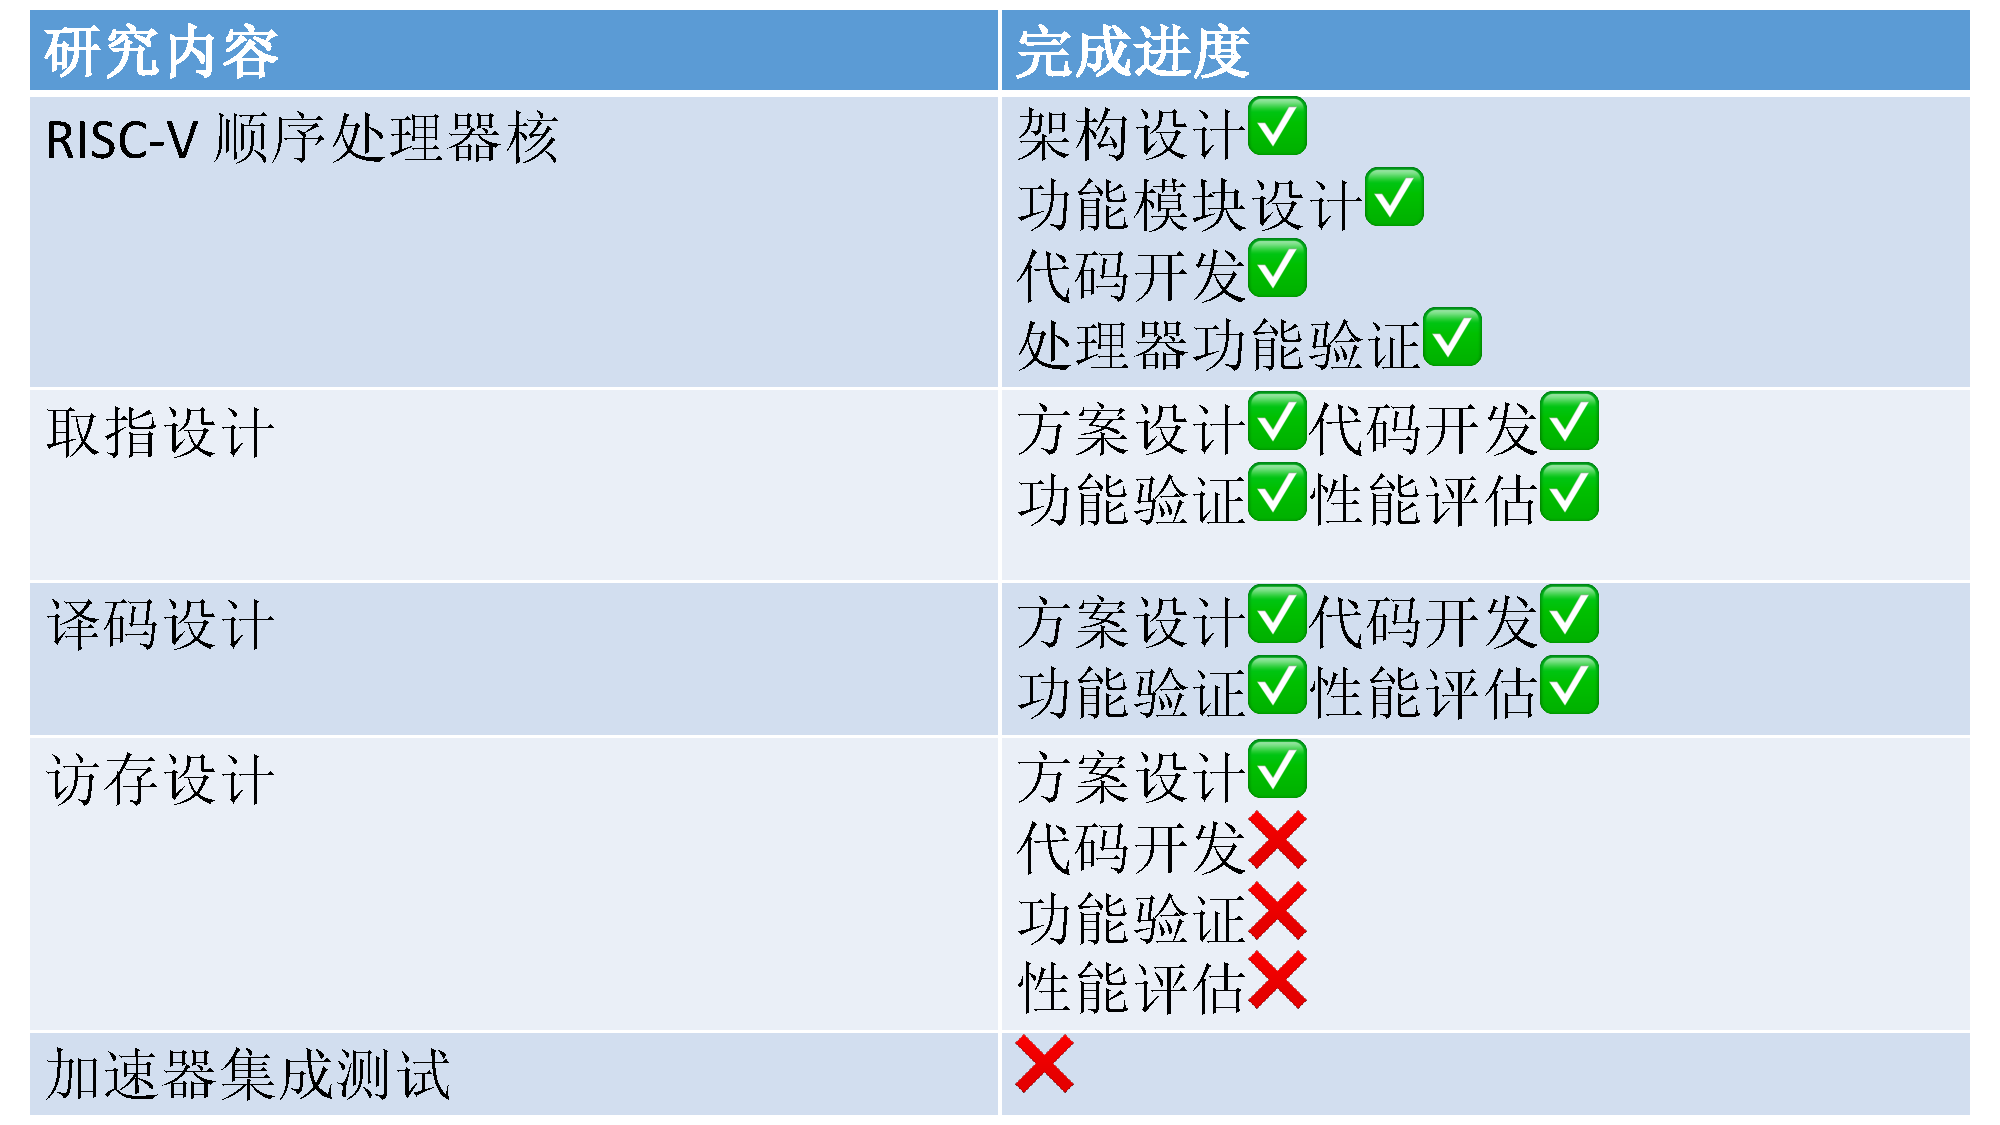
\includegraphics[width=\linewidth]{./images/study_progress.pdf}
  \caption{课题当前完成的部分及未完成的部分}
  \label{fig:study_progress}
\end{figure*}

% \begin{table}[ht]
%   \caption{A table arranging  images}
%   \begin{tabular}{c}
%   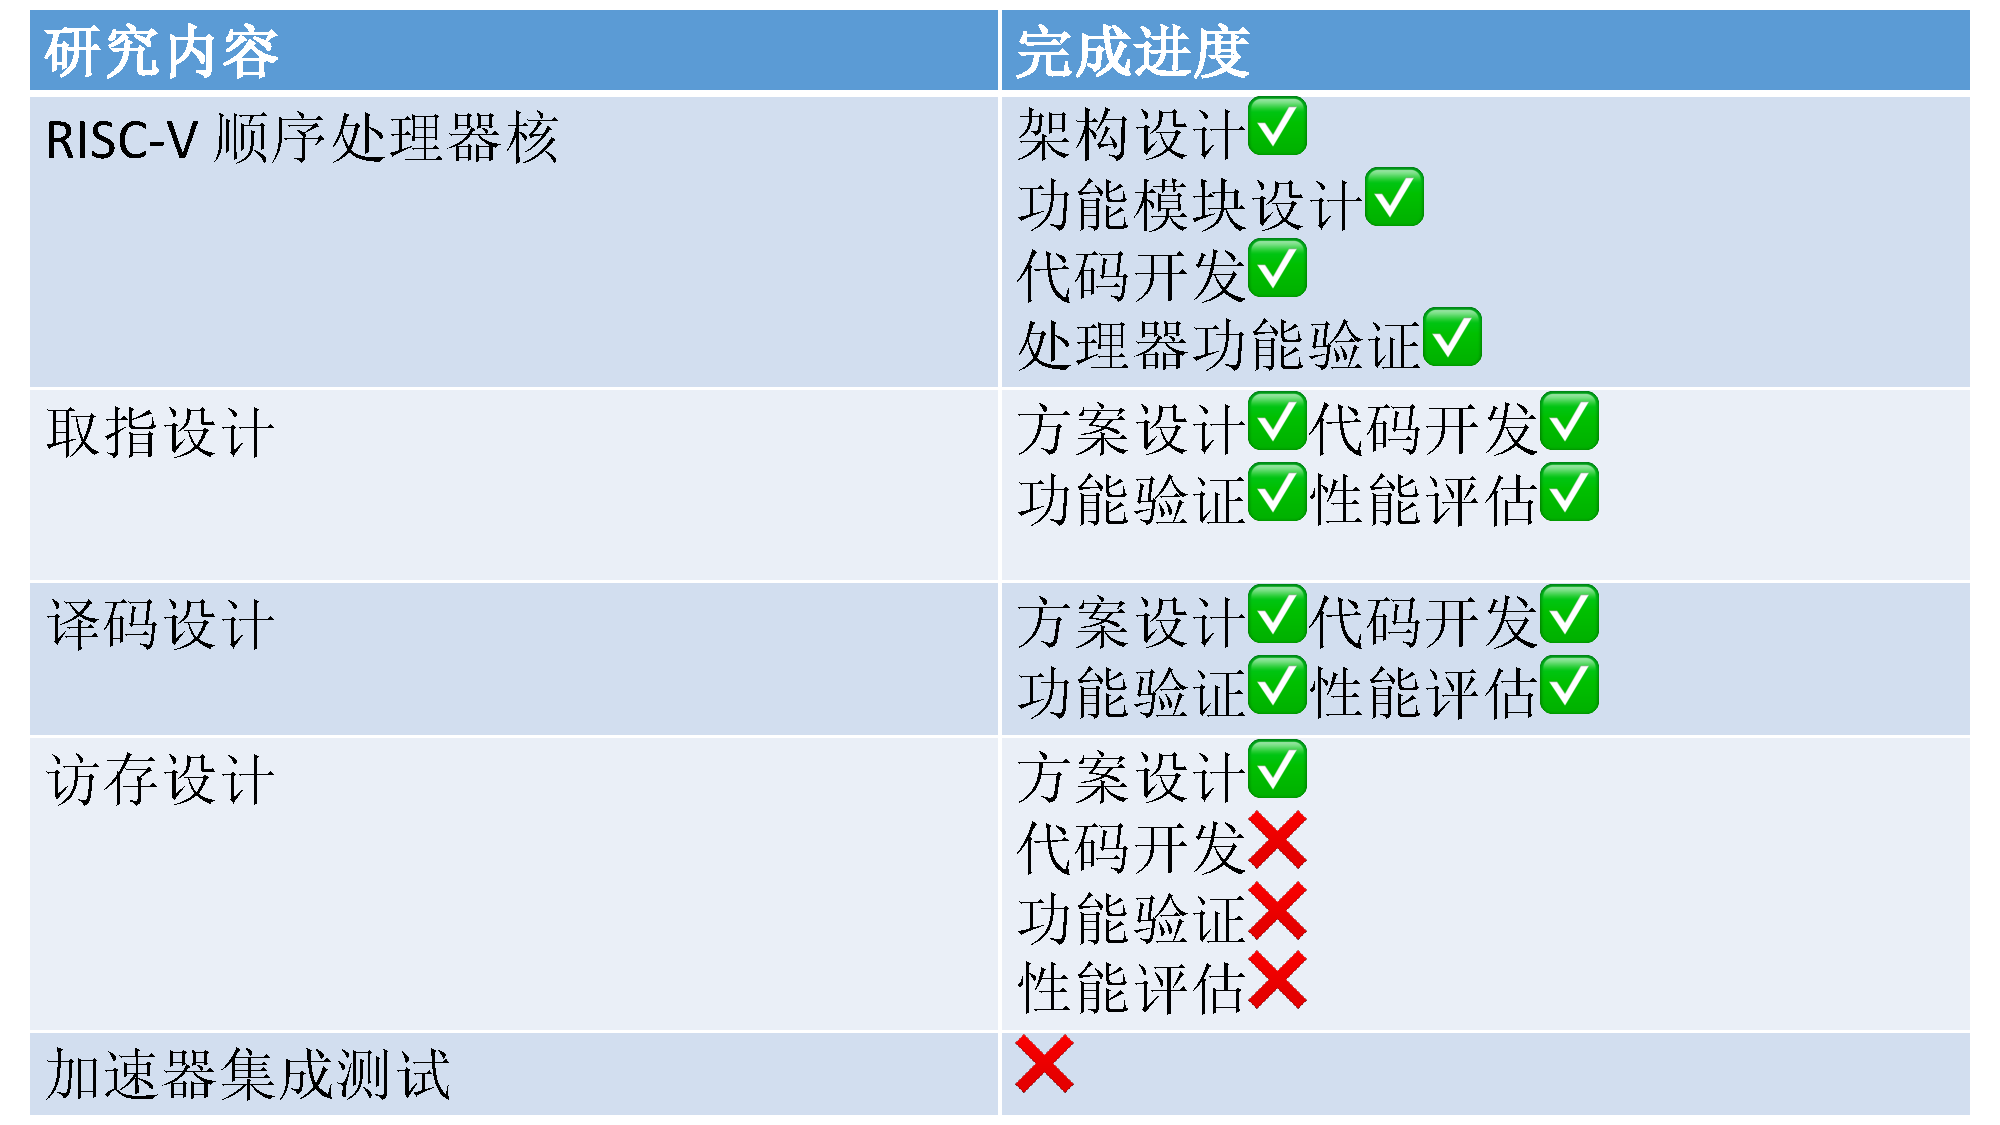
\includegraphics[scale=0.5]{./images/study_progress.pdf}\\
%   \end{tabular}
%   \label{tab:gt}
% \end{table}


% \begin{table}[H]
%   \caption{\textbf{table caption)}}
%   \centering
%     \begin{tabular}{cc}
%       \label{tab:pc_flash}
%       \toprule
%       a & b\\
%       \midrule 
%         c & d\\
%       \bottomrule
%   \end{tabular}
% \end{table}

\clearpage
\section{已完成内容}%
\subsection{技术路线}%
本课题的技术路线采用\textbf{先实现再优化}的思想。首先根据当前项目的资料分析了需要解决的问题;确定加速器调度问题的主要应用场景之后确定了微控制器的主要任务,并且在此基础上确定了微控制器采用顺序单发射架构、支持RISC-V 32IMC指令集,其中乘法指令集(M)是为了保证微控制器一定的计算性能、压缩指令集(C)则是压缩程序所占用的存储面积,保证应用程序能够存储。

微控制器功能特性确定之后,按照五级流水线架构对微处理器进行了实现,其中模块集级验证采用了testbench进行简单验证;微控制器系统级验证采用了Difftest框架进行验证,验证通过了所有的RISC-V TESTS测试集,在一定程度上保证了微控制器是正确实现了RISC-V手册规范的。

在处理器核功能正确的基础上,针对加速器调度的场景以及低功耗\cite{8106976}需求进行了优化设计,主要特现在:取指部分针对整数指令地址不对齐做了优化;译码部分实现了分支预测器以及地址重定向的仲裁;访存部分针对加速器配置信息下发做了优化。优化设计完成之后对微控制器再次进行Difftest测试,保证微控制器优化设计之后依然符合RISC-V手册规范、检查优化之后的微控制器设计是否取得了设计的性能提升。
% 最后,将微控制器集成到5G基带芯片内做功能测试,对微控制器的功能跟性能进行测试。
  
\clearpage
\subsection{研究方法}%
当前本课题已经实现了取指部分以及译码部分优化设计,针对访存部分的设计优化正在进行当中。
\subsubsection{取指部分}
\textbf{(a)问题提出}:由于5G基带芯片对于实时性的要求很高\cite{kim2020flexible},因此用于加速器调度的微控制器本身也需要满足实时性的设计。在这个前提下,微控制器不能使用Cache做指令存储,因为Cache会存在Cache Miss的问题\cite{duran2020energy},导致取指部分的时延不能保证,违反了实时性的要求,因此取指部分采用\textbf{ITCM}(Instruction Tightly Coupuled Memory)做指令存储。
ITCM由于需要匹配微控制器的速度,其容量不能做到很大,因此在设计微控制器架构的时候需要实现压缩指令集\cite{tabanelli2022optimizing},RISC-V手册规定其压缩指令(16 bits)跟整数指令(32 bit)在指令存储内部是混合存储的\cite{balas2021risc},因此引出了\textbf{整数指令跟压缩指令混合存储时整数指令的取指问题}\cite{scheipel2022moremcu},该问题具体表现为如下两点:
\begin{enumerate}
  \item 当整数指令取指地址不是2B对齐的时候,如何访问一次ITCM在一个cycle内完成整数指令的取指。
  \item 整数指令跟压缩指令在指令存储内混合存放,微控制器如何对从指令存储内取出的指令做边界判定,识别出每一条压缩指令跟整数指令。
\end{enumerate}

\textbf{(b)研究目标}:微控制器的取指部分需要实现在一个cycle内取出一条整数指令,并且完成整数指令跟压缩指令的识别并且在整数指令地址不对齐的时候完成对整数指令的拼接。其设计目标如图\ref{fig:if_design_features}所示。

\textbf{(c)设计方案}:取指部分采用\textbf{odd even ITCM 跟取指FIFO}来实现上述的设计目标。
\begin{figure}
  \centering
  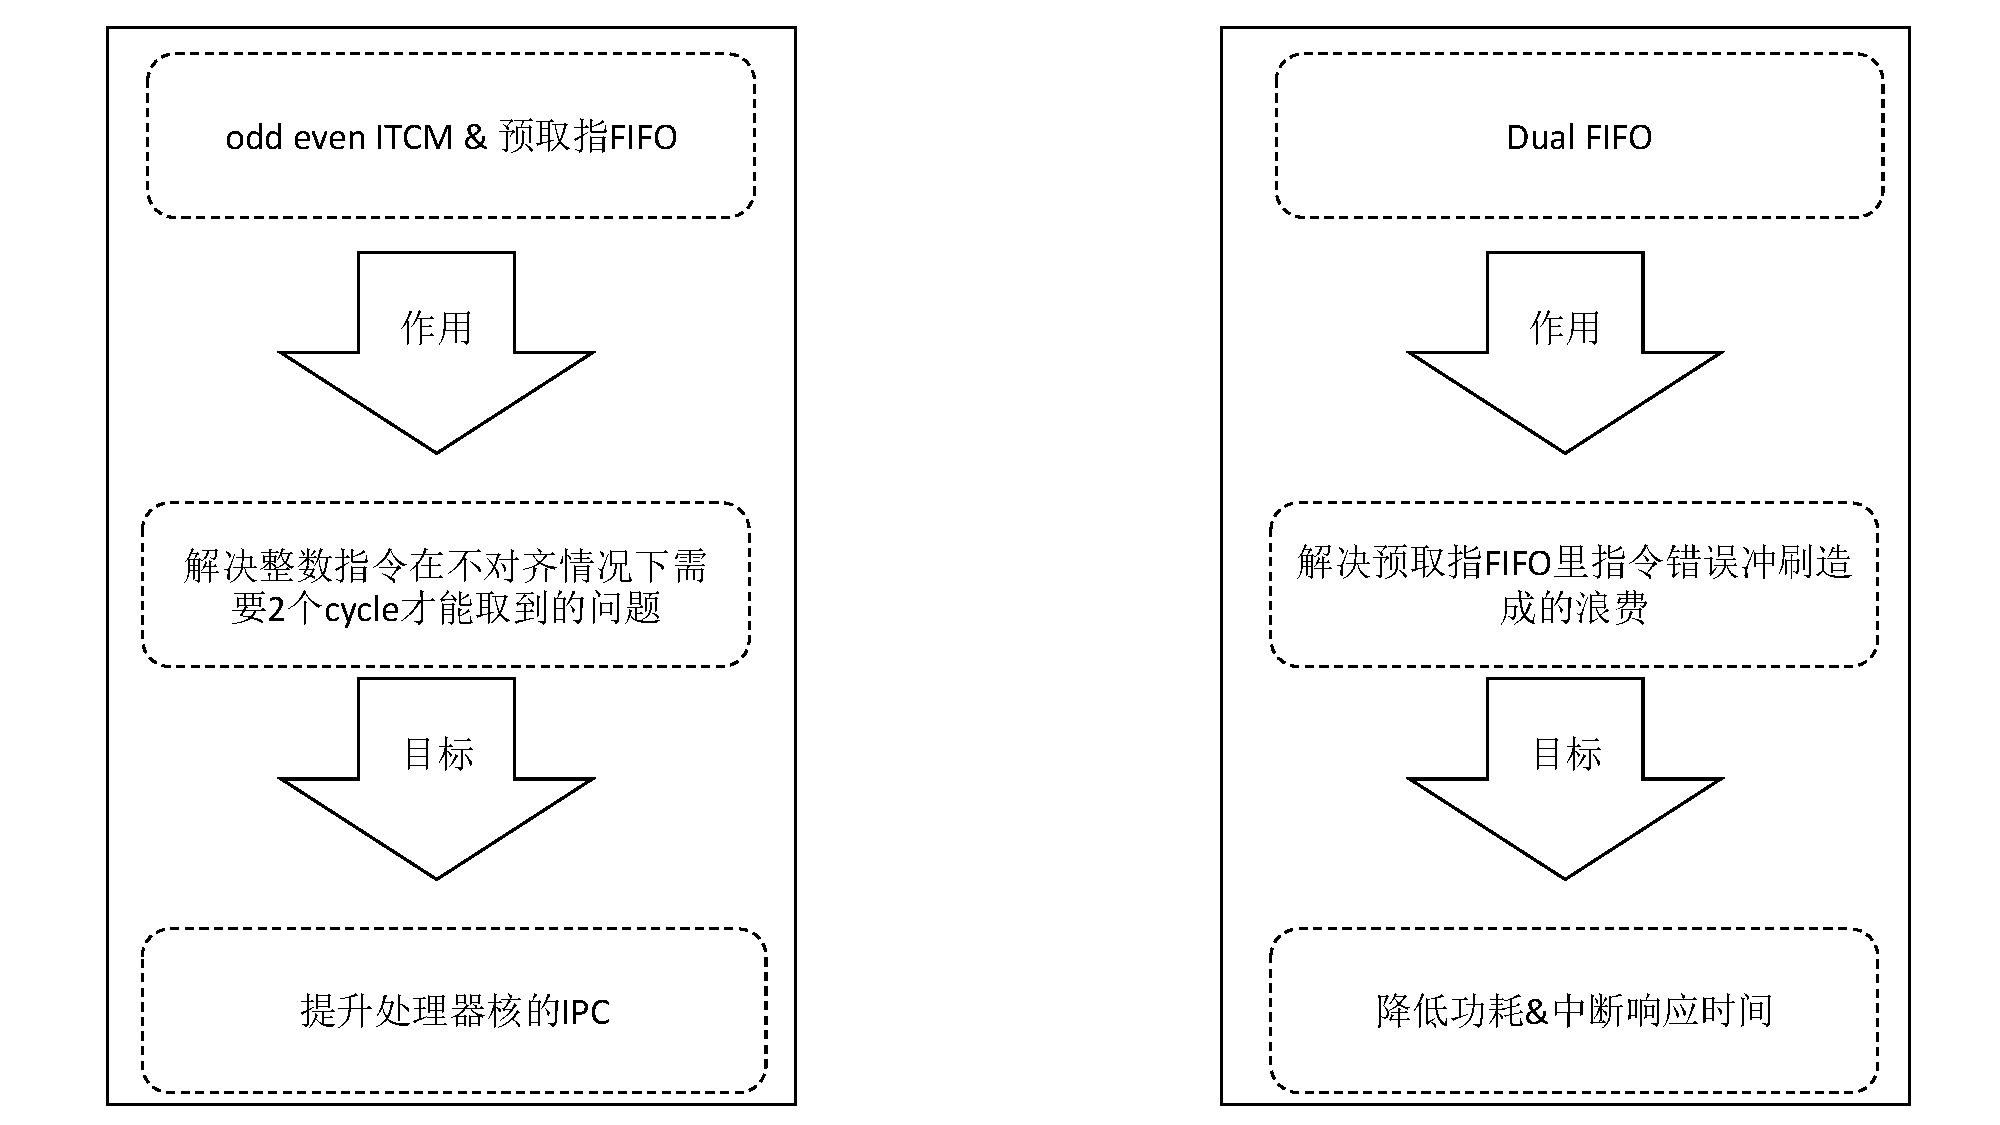
\includegraphics[width=0.8\linewidth]{./images/if_design_features.pdf}
  \caption{采用odd even ITCM跟取指FIFO解决整数指令跟压缩指令混合存储时整数指令取指问题}
  \label{fig:if_design_features}
\end{figure}

\begin{itemize}
  \item \textbf{odd even ITCM}:
    指令的取指地址可能是4B对齐也可能是2B对齐的,地址2B对齐的时候需要访问两次ITCM才可以才可以从ITCM里取出整数指令的高16bits跟低16bits,再通过拼接电路完成整数指令的拼接。\\ 
    当地址是连续递增的时候可以采用\textit{leftover buffer}存储上一次访问ITCM得到的高16 bits数据,如图\ref{fig:if_leftover_buffer}所示。当地址2B对齐的时候可以利用\textit{leftover buffer}里的内容实现整数指令的拼接。\textit{但是这种方法在地址出现跳转时会失效}。
    \begin{figure}[htbp]
      \centering
      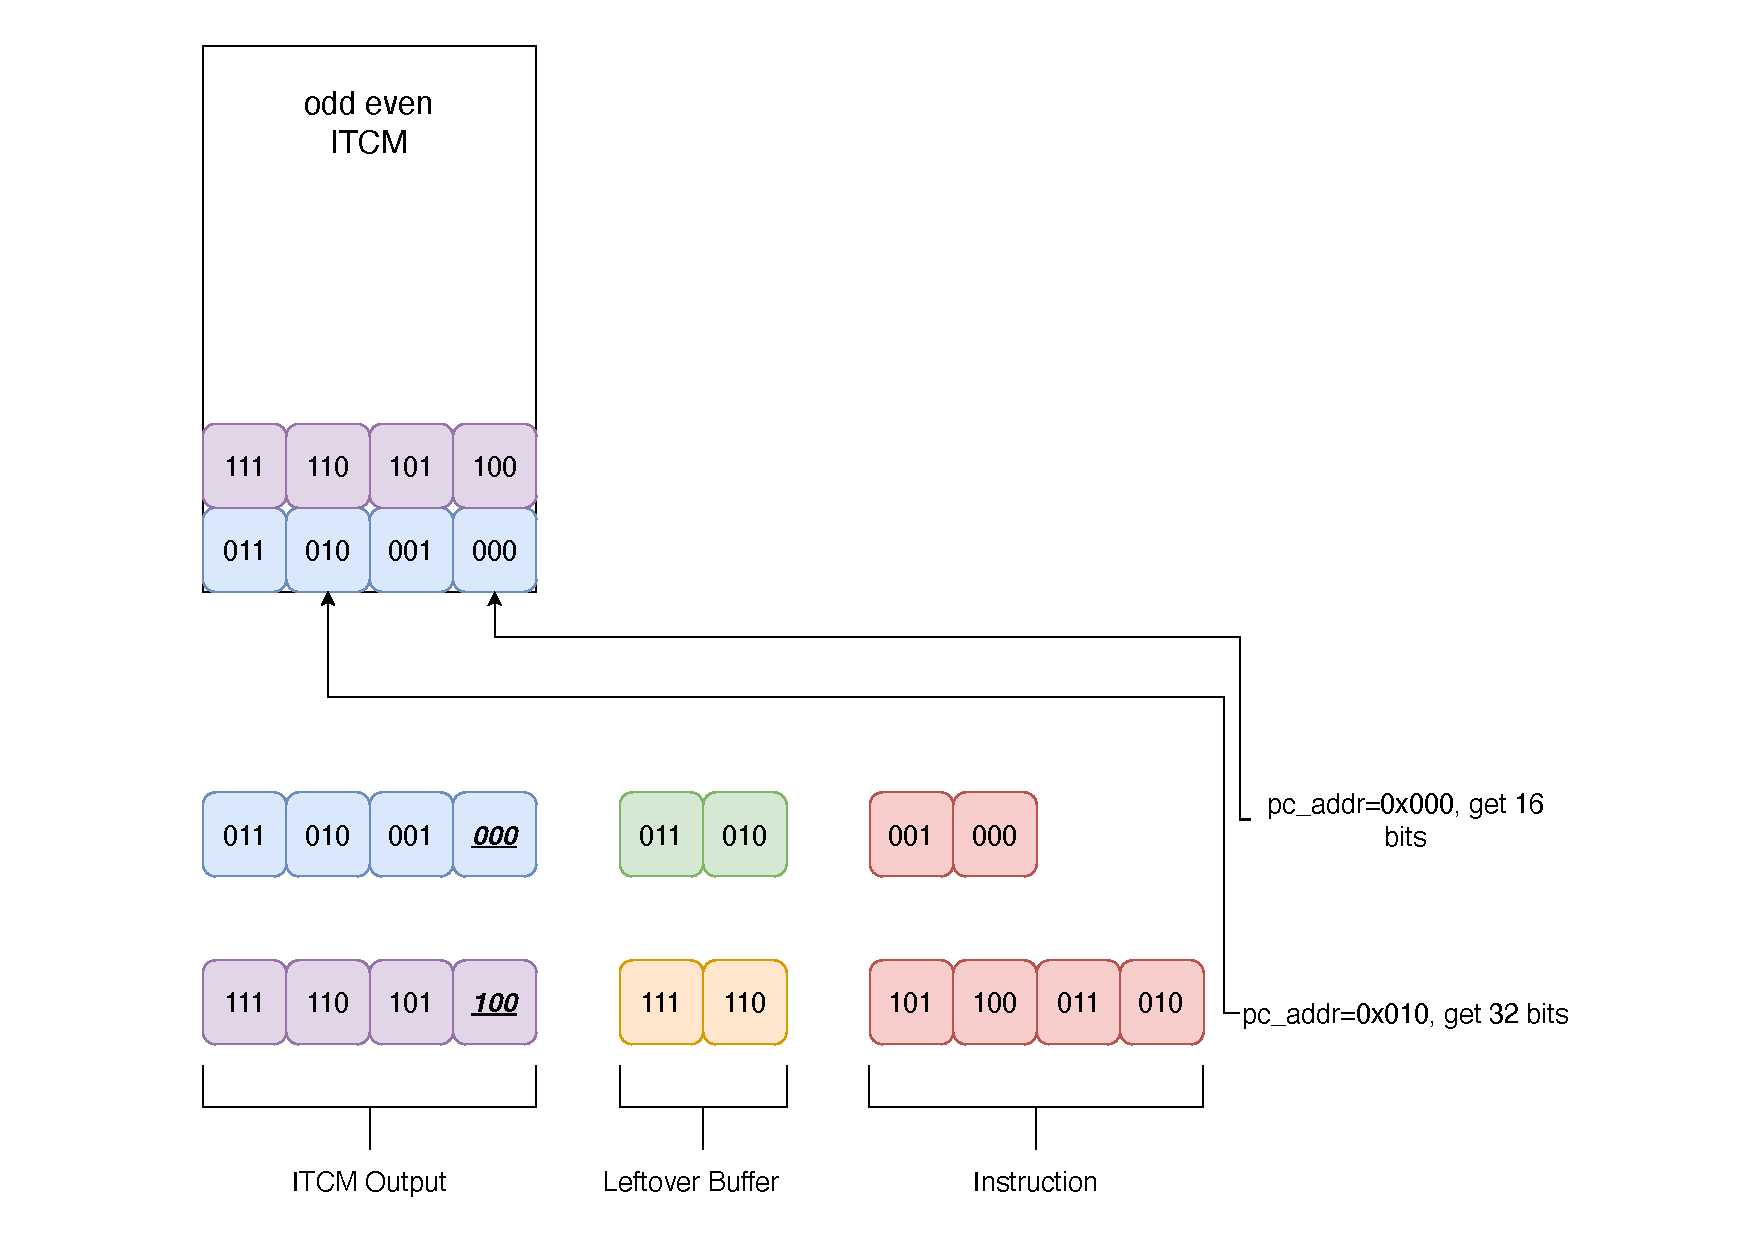
\includegraphics[width=0.8\linewidth]{./images/if_leftover_buffer.pdf}
      \caption{采用leftover buffer来实现整数指令的拼接}
      \label{fig:if_leftover_buffer}
    \end{figure}
    本课题采用\textit{odd even ITCM}可以解决指令跳转后出现地址不是4B对齐时的整数指令的取指问题。其核心思想在于\textbf{将ITCM分为odd, even}两部分,两部分可以独立的访问。当地址不是4B对齐的时候,\textit{even ITCM}访问地址比\textit{odd ITCM}高一位,并且将\textit{even ITCM}里的数据当作高16 bits,\textit{odd ITCM}里的数据当低16 bits完成指令的拼接;当地址是4B对齐的时候,两块ITCM的访问地址一样,并且\textit{even ITCM}的数据当作低16 bits完成指令的拼接。具体操作原理如图\ref{fig:2bank_ITCM}所示。

    \begin{figure}[htbp]
      \centering
      \subfloat[取指地址不是4B对齐时odd even ITCM的访存地址不同]{
        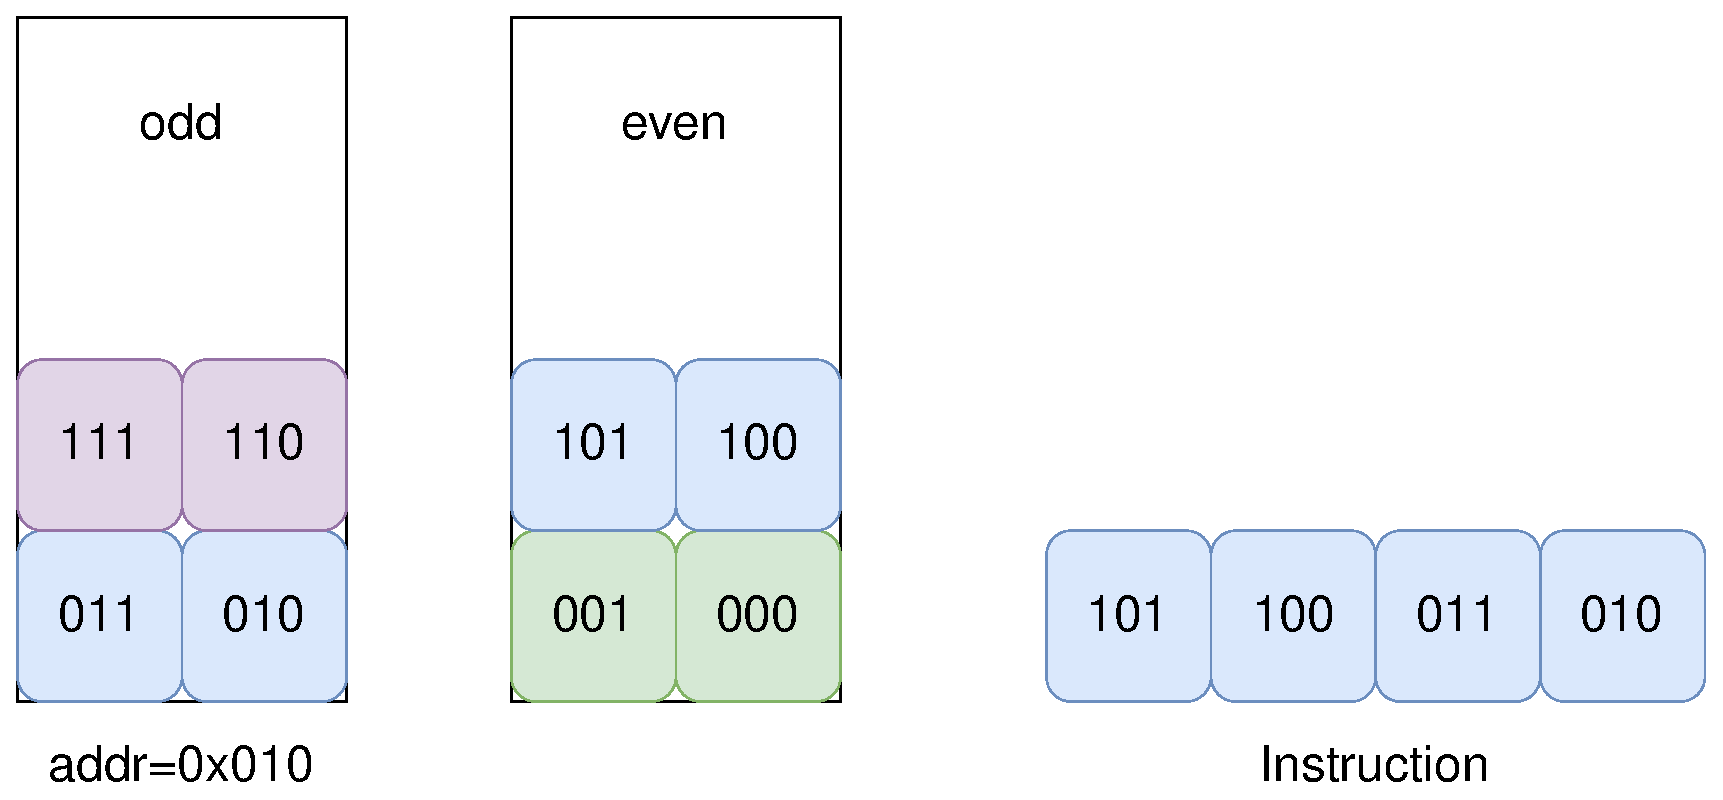
\includegraphics[width=0.8\linewidth]{./images/2bank_1.eps}
      }\\
      \subfloat[取指地址是4B对齐时odd even ITCM的访存地址相同]{
        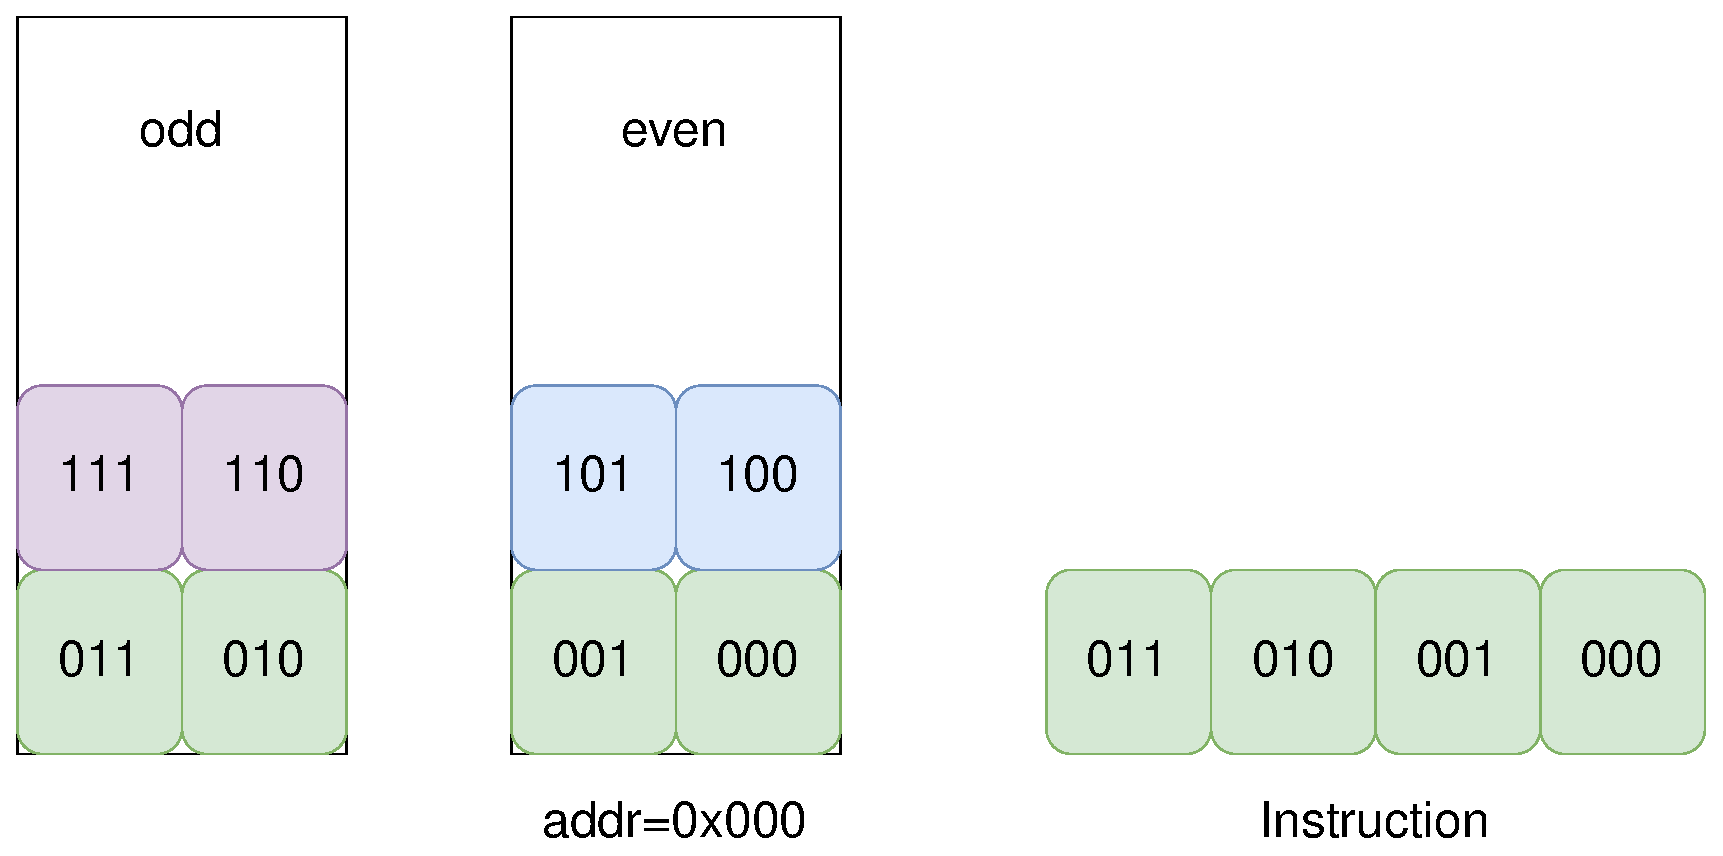
\includegraphics[width=0.8\linewidth]{./images/2bank_2.eps}
      }
      \caption{odd even ITCM解决整数指令地址不对齐的问题}
      \label{fig:2bank_ITCM}
    \end{figure}
  \item \textbf{取指FIFO}

    在访问ITCM的时候,只能根据地址是否是4B对齐控制访问ITCM的动作,但是从ITCM里取出的指令可能的组合有如下五种情况\cite{1022693926.nh}。
    \begin{enumerate}
      \item 取出的32 bits数据是一条整数指令
      \item 取出的32 bits数据是两条压缩指令
      \item 取出的32 bits数据是一条压缩指令跟一条整数指令的低16 bits
      \item 取出的32 bits数据是一条整数指令高16 bits跟一条压缩指令
      \item 取出的32 bits数据是一条整数指令高16 bits跟一条整数指令低16 bits
    \end{enumerate}
为了判断具体指令的类型,需要复杂的硬件电路来从上述五种可能的情况里判断出取出的数据具体属于哪种类型,然后根据当前指令的类型来更新下一次取指地址的值。这会导致如下的缺陷:
\begin{enumerate}
  \item 取指级的周期变长:取出来的数据需要复杂的硬件电路才可以判断出指令的类型,这会增减组合逻辑电路的延时;下一次取指的地址需要根据当前指令的类型选择加4或者加2。
  \item 在可能的组合2、4中,高16 bits的压缩指令会被重复取出,因为这两种情况下取指地址会加2,导致了额外的访存功耗。
\end{enumerate}
    基于上述硬件电路的缺点,本课题提出了\textit{5*16}的取指FIFO,用于存储从ITCM中取出的数据、完成指令类型的判断以及整数指令的拼接,其结构如图\ref{fig:itcm_fifo}所示;其操作逻辑如下:

    \begin{figure}[htbp]
      \centering
      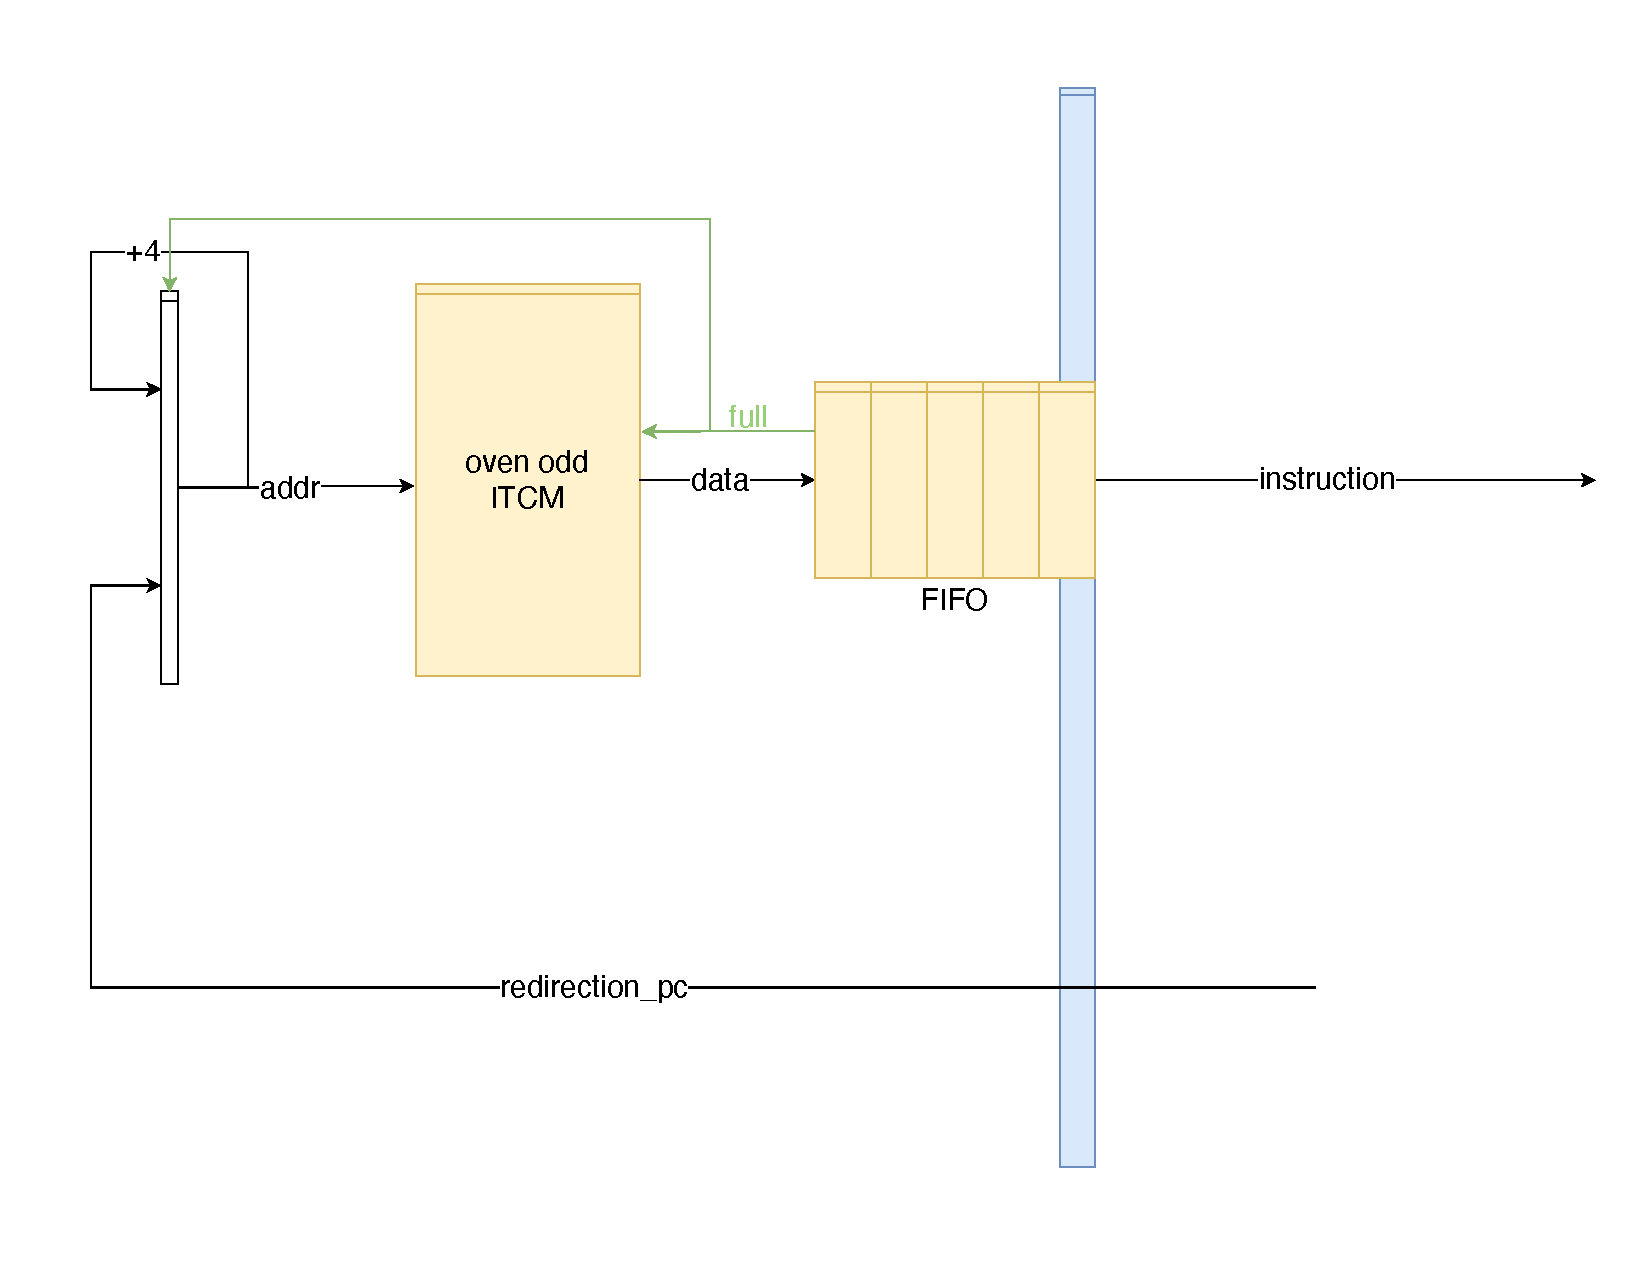
\includegraphics[width=0.7\linewidth]{./images/itcm_fifo.pdf}
      \caption{odd even ITCM跟取指FIFO结构图}
      \label{fig:itcm_fifo}
    \end{figure}
\begin{enumerate}
  \item FIFO总容量为5,表示其内部的5个16 bits的寄存器。容量设计为5是为了避免写入到FIFO的时候出现overflow。
  \item 从ITCM中每次都会得到32 bits的数据,当FIFO容量$\le 3$的时候FIFO允许被写入,取出的32 bits数据会被push到FIFO中。
  \item 当译码级没有被stall的时候,每个cycle会译码一条指令,译码的时候会判断FIFO头部寄存器的低2 bits是否是\textit{11}。根据RISC-V规定,指令低2 bits如果是11则表示当前指令是一条整数指令,此时会从FIFO头部pop出2个16bits的数据,即一条整数指令;反之如果低2 bits不是11,则说明当前指令是一条压缩指令,此时只需要pop出FIFO头部一条指令即可。
\end{enumerate}
  \item \textbf{Dual FIFO}:\textit{通过odd even ITCM跟取指FIFO的设计起到了避免多次访问ITCM(降低了存储器的动态访问功耗\cite{9286538})、提高整数指令跟压缩指令的取指效率。}但是取指FIFO面对流水线冲刷的时候,都需要将所有预取的指令都冲刷掉,但是流水线冲刷可能是错误的,例如分支预测错误。

    因此本课题针对所有指令流跳转的场景,提出了\textit{Dual FIFO}的设计,其结构如图\ref{fig:if_dual_fifo}所示:当指令流需要跳转的时候,当前FIFO的指令不会立刻被出冲刷掉,跳转后的指令流对应的指令会被暂存到另一个空闲的取指FIFO中。
    \begin{enumerate}
      \item 当指令流跳转被判断正确的时候,之前的取指FIFO才会被真正冲刷掉。
      \item 当指令流跳转被判断错误的时候,会直接从之前的取指FIFO里继续执行,避免了指令的浪费以及取指的延时。
    \end{enumerate}
  
\end{itemize}

\begin{figure}[htbp]
  \centering
  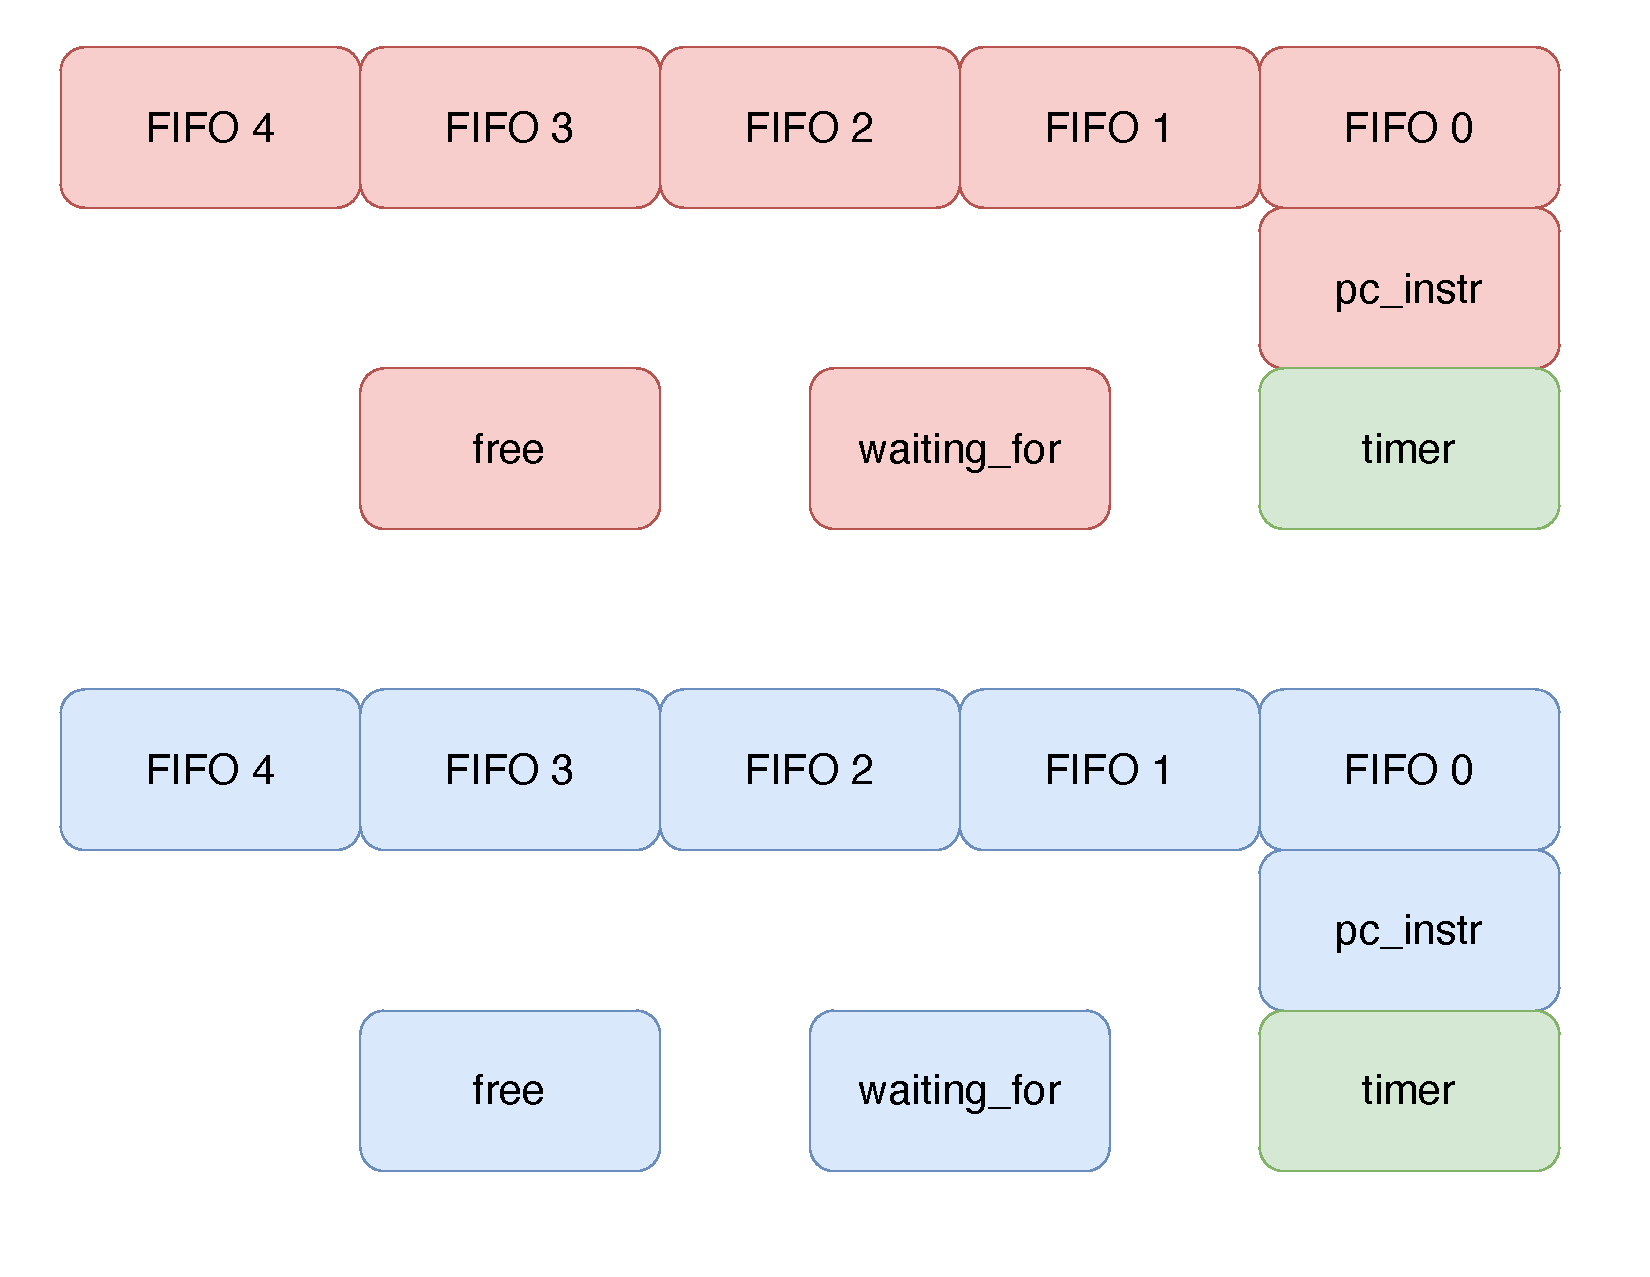
\includegraphics[width=0.6\linewidth]{./images/if_dual_fifo.pdf}
  \caption{Dual FIFO的硬件设计}
  \label{fig:if_dual_fifo}
\end{figure}

\subsubsection{译码部分}
\textbf{(a)问题提出}:
在指令流水中,可能会存在分支跳转指令(如RISC-V BEQ指令),导致指令流发生跳转\cite{al2020hybrid}。如果不对分支指令跳转进行预测,那么微控制器就会浪费时间去执行错误的指令,造成了微控制器IPC的降低\cite{arul2020design};此外微控制器指令流中有很多情况会导致指令重定向,例如分支预测、外部中断、异常处理、系统复位等情况\cite{benila2022plan},这些重定向都涉及到取指地址的改变,需要有一种仲裁机制来保证取指地址更新满足所有的重定向的情况\cite{choudhury2022optimized}。

\textbf{(b)研究目标}:
译码级需要支持静态分支预测器,来提供基础的分支预测的能力以及避免微控制器功耗面积过大\cite{park2019branch};此外译码级需要对系统可能遇到的所有的重定向的情况做仲裁,然后将重定向地址发送给取指级\cite{miyazaki2020rvcorep}。译码级研究目标如图\ref{fig:id_design_features}所示。

\begin{figure}[htbp]
  \centering
  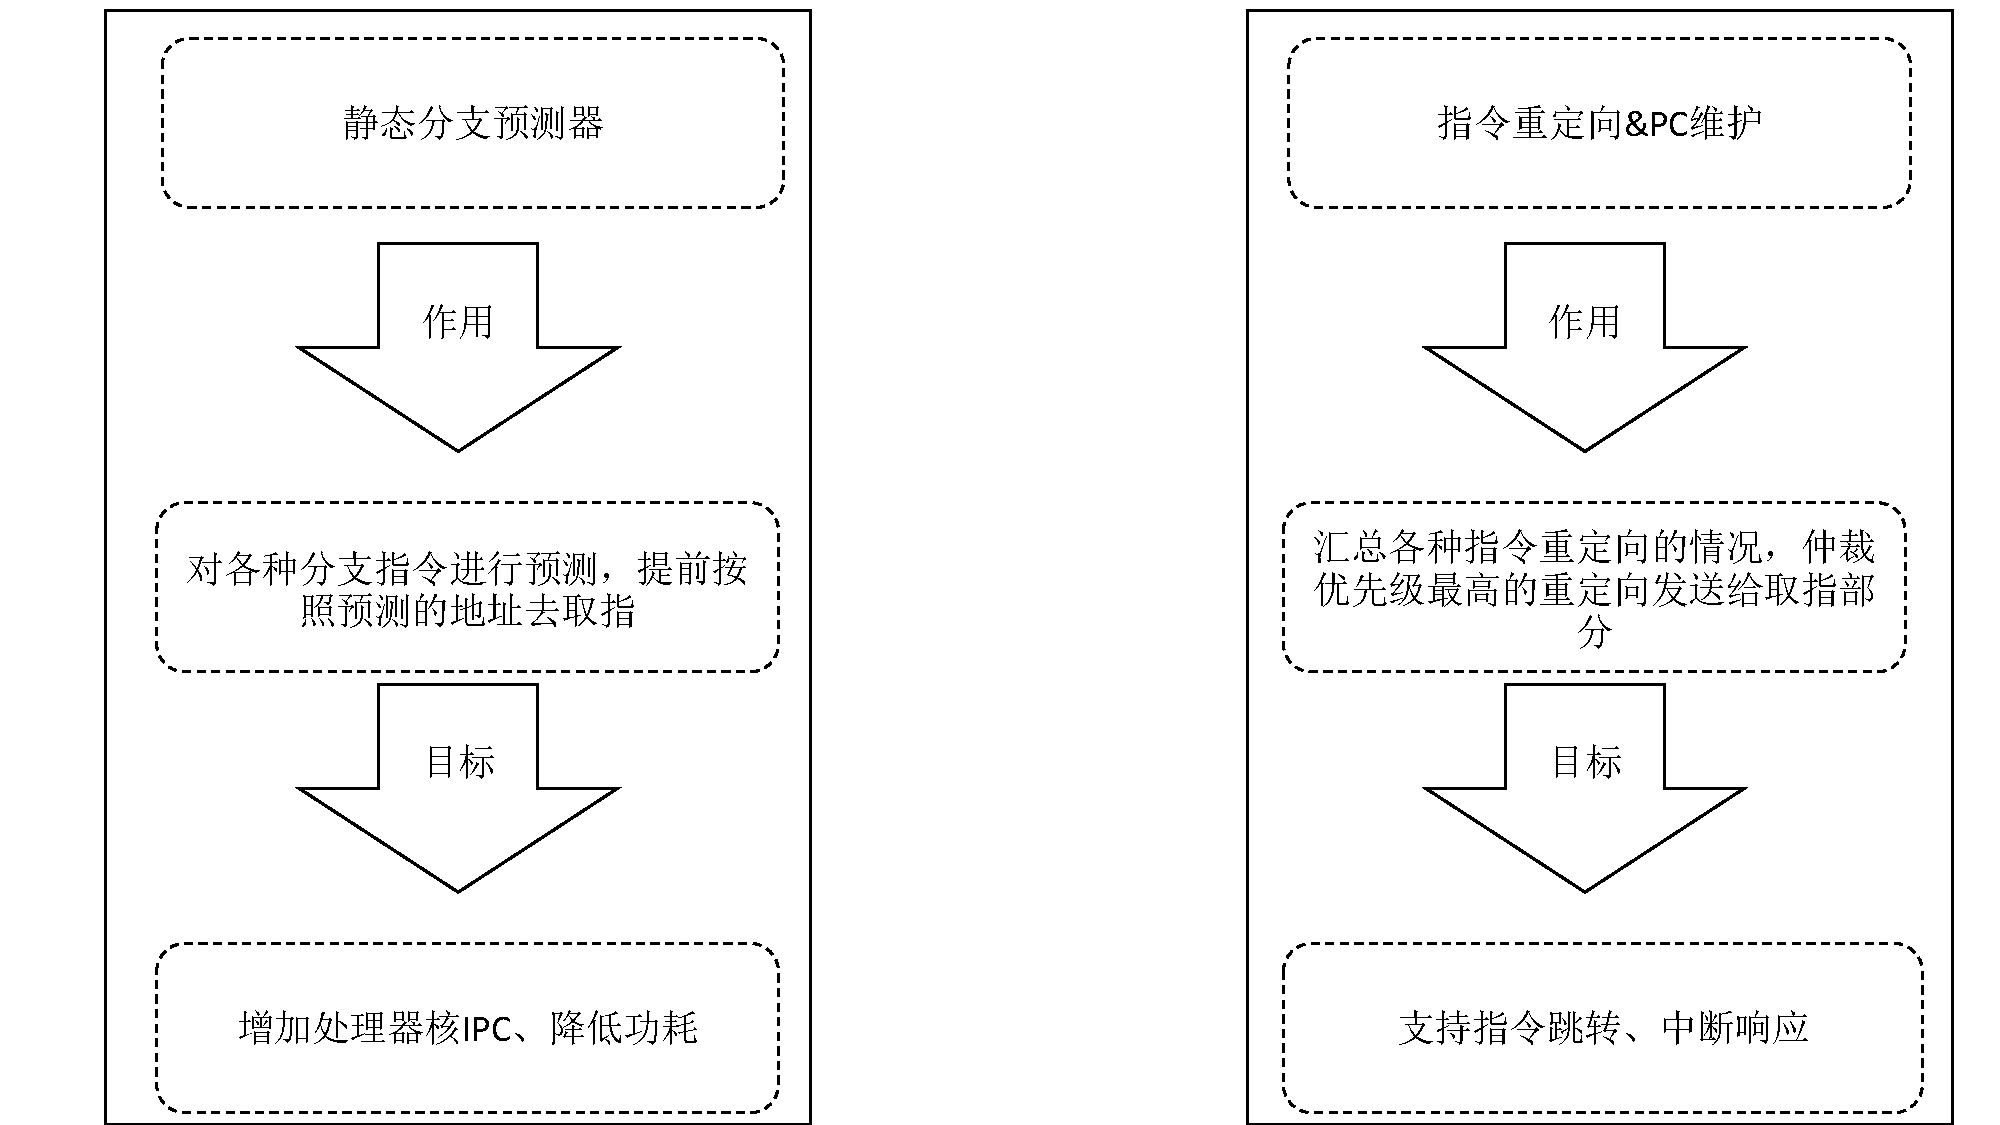
\includegraphics[width=0.8\linewidth]{./images/id_design_features.pdf}
  \caption{采用静态分支预测器提高微控制器IPC;在译码级实现指令重定向的仲裁}
  \label{fig:id_design_features}
\end{figure}

\textbf{(c)设计方案}:
  \begin{itemize}
    \item \textbf{静态分支预测器}
      由于本课题设计的微控制器属于嵌入式领域,要求低功耗及低面积,所以在考虑其分支预期的时候,没有考虑采用动态分支预测器的方案;因此本课题设计了静态分支预测器来对RISC-V的3类分支指令做预测,其预测的规则如下:
      \begin{enumerate}
        \item JAL指令:预测$100\%$跳转,其跳转地址直接有静态分支预测器遇得到到。
        \item JALR指令:预测$100\%$跳转,其跳转地址直接有静态分支预测器计算得到(由于JALR指令需要读取通用寄存器组RF(Register File)的值才可以计算出跳转地址,如果将静态分支预测器设置在取指级则必须将所有的通用寄存器值全部Bypass到取指级,这将大大增加连线的面积,相应的连线延时也会导致取指级成为关键路径。因此本课题将分支预测器放置在译码级,以$2.31\%$IPC代价换来了更小的面积、更高的频率以及更低的功耗)。
        \item Branch Type指令:RISC-V一共有6条条件跳转指令,该类型指令是否跳转取决于寄存器值比较的结果,因此采用静态分支预测器对跳转跳转预测准确率无法达到$100\%$,采用FTBN(forward taken, backward not taken)的策略对条件跳转指令进行预测,能够达到$75\%$以上的准确率。
      \end{enumerate}
      之所以在微控制器中采用静态分支预测器的另一个原因在于:微控制器的流水线很浅,分支指令及时在执行级被计算出结果,也仅仅过了2个cycle,最多产生2条错误的指令;因此对于MCU这样的浅流水线处理器来说,预测准确率对于CPI(Clock per Instruction)的影响其实很低,图\ref{fig:sbp_cpi}显示了预测准确率对于五级流水线的微控制器CPI的影响。
    \begin{figure}[htbp]
      \centering
      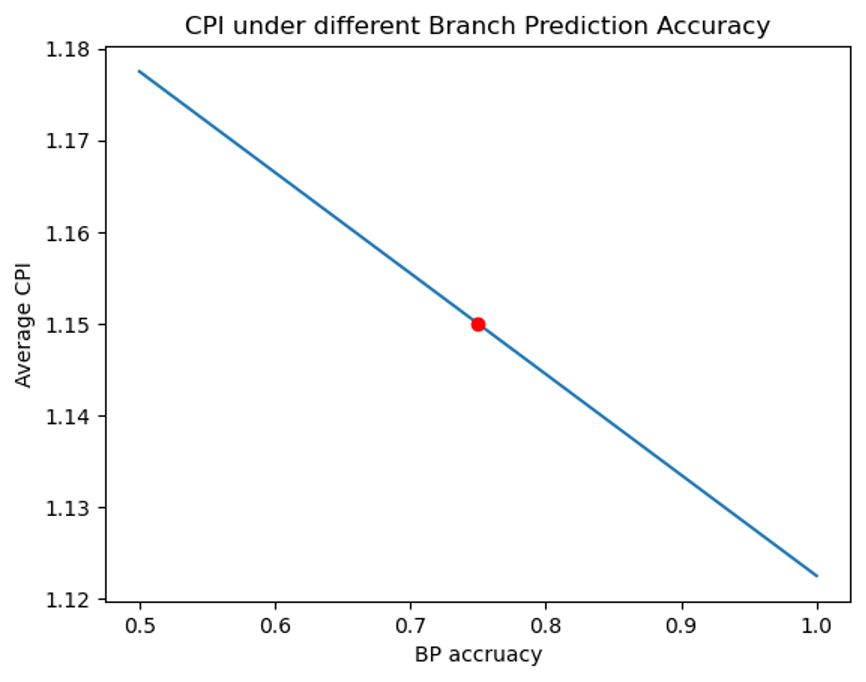
\includegraphics[width=0.7\linewidth]{./images/sbp_cpi.png}
      \caption{分支预测器准确率对五级流水线微控制器CPI的影响}
      \label{fig:sbp_cpi}
    \end{figure}

    \item \textbf{重定向\&PC维护}:
      本课题所设计的微控制器,其取指级只负责维护\textit{顺序取指地址},每条指令跟其对应的PC相对应实在译码级完成的,RISC-V中的AUIPC, JAL等指令的计算需要用到指令对应的PC。

      % 在此基础上,所有重定向地址的仲裁也被放在了译码级,一方面是因为译码级维护了每条指令跟其PC的对应关系;另一方面是为了简化取指级的PC更新逻辑,避免取指级成为关键路径。译码级所需要维护的所有重定向类型及对应的PC更新逻辑如表\ref{tab:pc_flash}所示:

% \begin{table}[H]
%   \caption{\textbf{PC重定向及PC更新逻辑, PTNT(Prediction Taken but Not Taken), SBP(Static Branch Predictor), MERT(RISC-V Machine Return Instruction)}}
%   \centering
%     \begin{tabular}{cc}
%       \label{tab:pc_flash}
%     \toprule
%     重定向场景 & PC更新\\
%     \midrule 
%       系统复位 & PC=0x80000000\\
%       中断异常 & PC=CSR.mtvec\\
%       PTNT and JAL & PC=PC\_NEXT\\
%       PTNT & PC=SBP\_PC\\
%       ALU Taken & PC=ALU\_PC\\
%       SBP Taken & PC=SBP\_PC\\ 
%       MRET & PC=CSR.mepc\\
%     \bottomrule
%   \end{tabular}
% \end{table}

  \end{itemize}  
\subsection{阶段性工作总结}
阶段性工作总结  
  目前微控制器所有的基础设计及优化设计都已经完成了方案论证、代码编写、设计验证的工作。
  目前译码级所有的功能部件如图\ref{fig:id_top}所示,译码级所有的功能部件已经完成了方案设计、代码编写以及功能验证。

    \textit{odd even ITCM的提出,减少了压缩指令的重复访存、减少了整数指令的重复访存及取指时延。}
    \textit{取指FIFO的提出,解决了指令混合存储时指令的边界判定问题,避免了复杂的组合判断电路的时延,减少了取指级的周期。}
    \textit{Dual FIFO的提出,可以减少$50.7\%$的ITCM访存、$31.7\%$的NOP指令导致的冲刷、$26.7\%$的程序返回的cycle数。减少了程序的执行时间、提升了处理器的效率,更高效地完成加速器调度任务;减少了无效指令进入流水线,减少了处理器时间,降低了处理器的功耗\cite{9613880}}

  \textit{静态分支预测器的提出,降低了$4.74\%$的CPI,减少了无效指令进入流水线,提高了微控制器的执行效率、降低了微控制器的功耗}
  \begin{figure}[htbp]
    \centering
    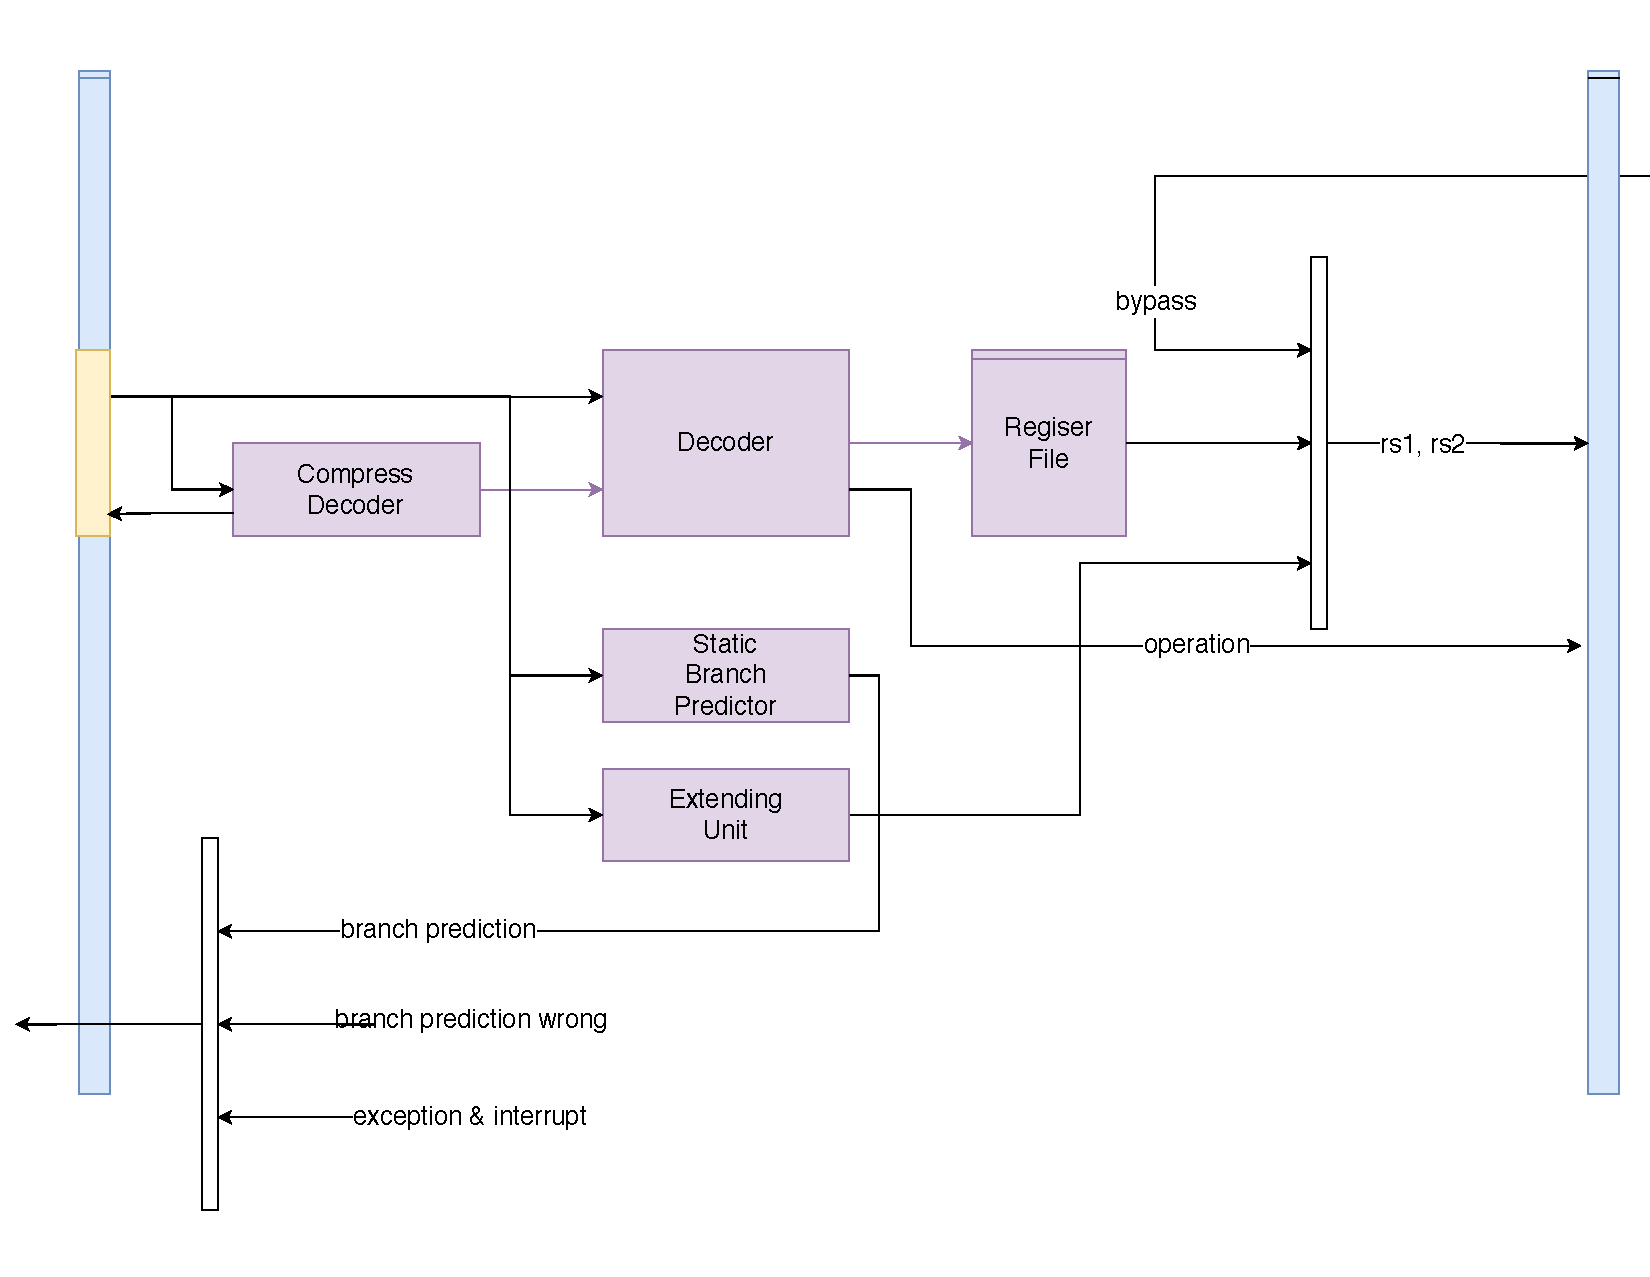
\includegraphics[width=0.8\linewidth]{./images/id_top.pdf}
    \caption{译码级功能部件逻辑框图}
    \label{fig:id_top}
  \end{figure}

\clearpage
\section{未来工作计划}%
\subsection{当前工作总结}

本课题当前完成的主要工作如下所示:
\begin{itemize}
  \item 处理器核架构定义、设计、代码编写、处理器核功能验证、Spyglass检查、DC综合,能够运行C程序。
  \item 取指部分针对中断响应、低功耗等需求,提出了2 Bank ITCM,Dual FIFO等创新设计\cite{10163410}。
  \item 译码部分实现了静态分支预测器及指令流跳转控制逻辑,支持程序流跳转及中断跳转。
  \item 访存部分按照RISC-V ISA规范,实现了8条访存指令的功能。
  \item 低功耗设计方面:
  \begin{itemize}
    \item 取指部分避免了压缩指令多次访问ITCM、FIFO冲刷浪费预取指令
    \item 执行时减少了Nop指令的产生,降低了处理器执行时间
  \end{itemize}
  \item 发表了一篇专利《由处理器执行的指令读取方法及相关产品》
\end{itemize}

\subsection{未来工作安排}

针对一开始开题时的计划,本课题目前还有如下三部分的问题需要解决:
\begin{enumerate}
  \item 需要增加对加速器寄存器进行配置的支持,主要体现在改进微控制器的访存模块,支持通过AXI总线从Config Memory读取配置信息、通过AXI总线向加速器写入配置信息。
  \item 实现WFI指令\cite{agarwal2019low},基于5G基带芯片低功耗的考虑,微控制器需要在基带芯片低负载的情况下通过Clock Gating进入睡眠模式以节约动态功耗\cite{venkatesan2019design}。
  \item 对优化后的微控制器做集成性能分析。
\end{enumerate}

本课题具体的工作计划安排如图\ref{fig:job_plan}所示:
\begin{figure}[htbp]
  \centering
  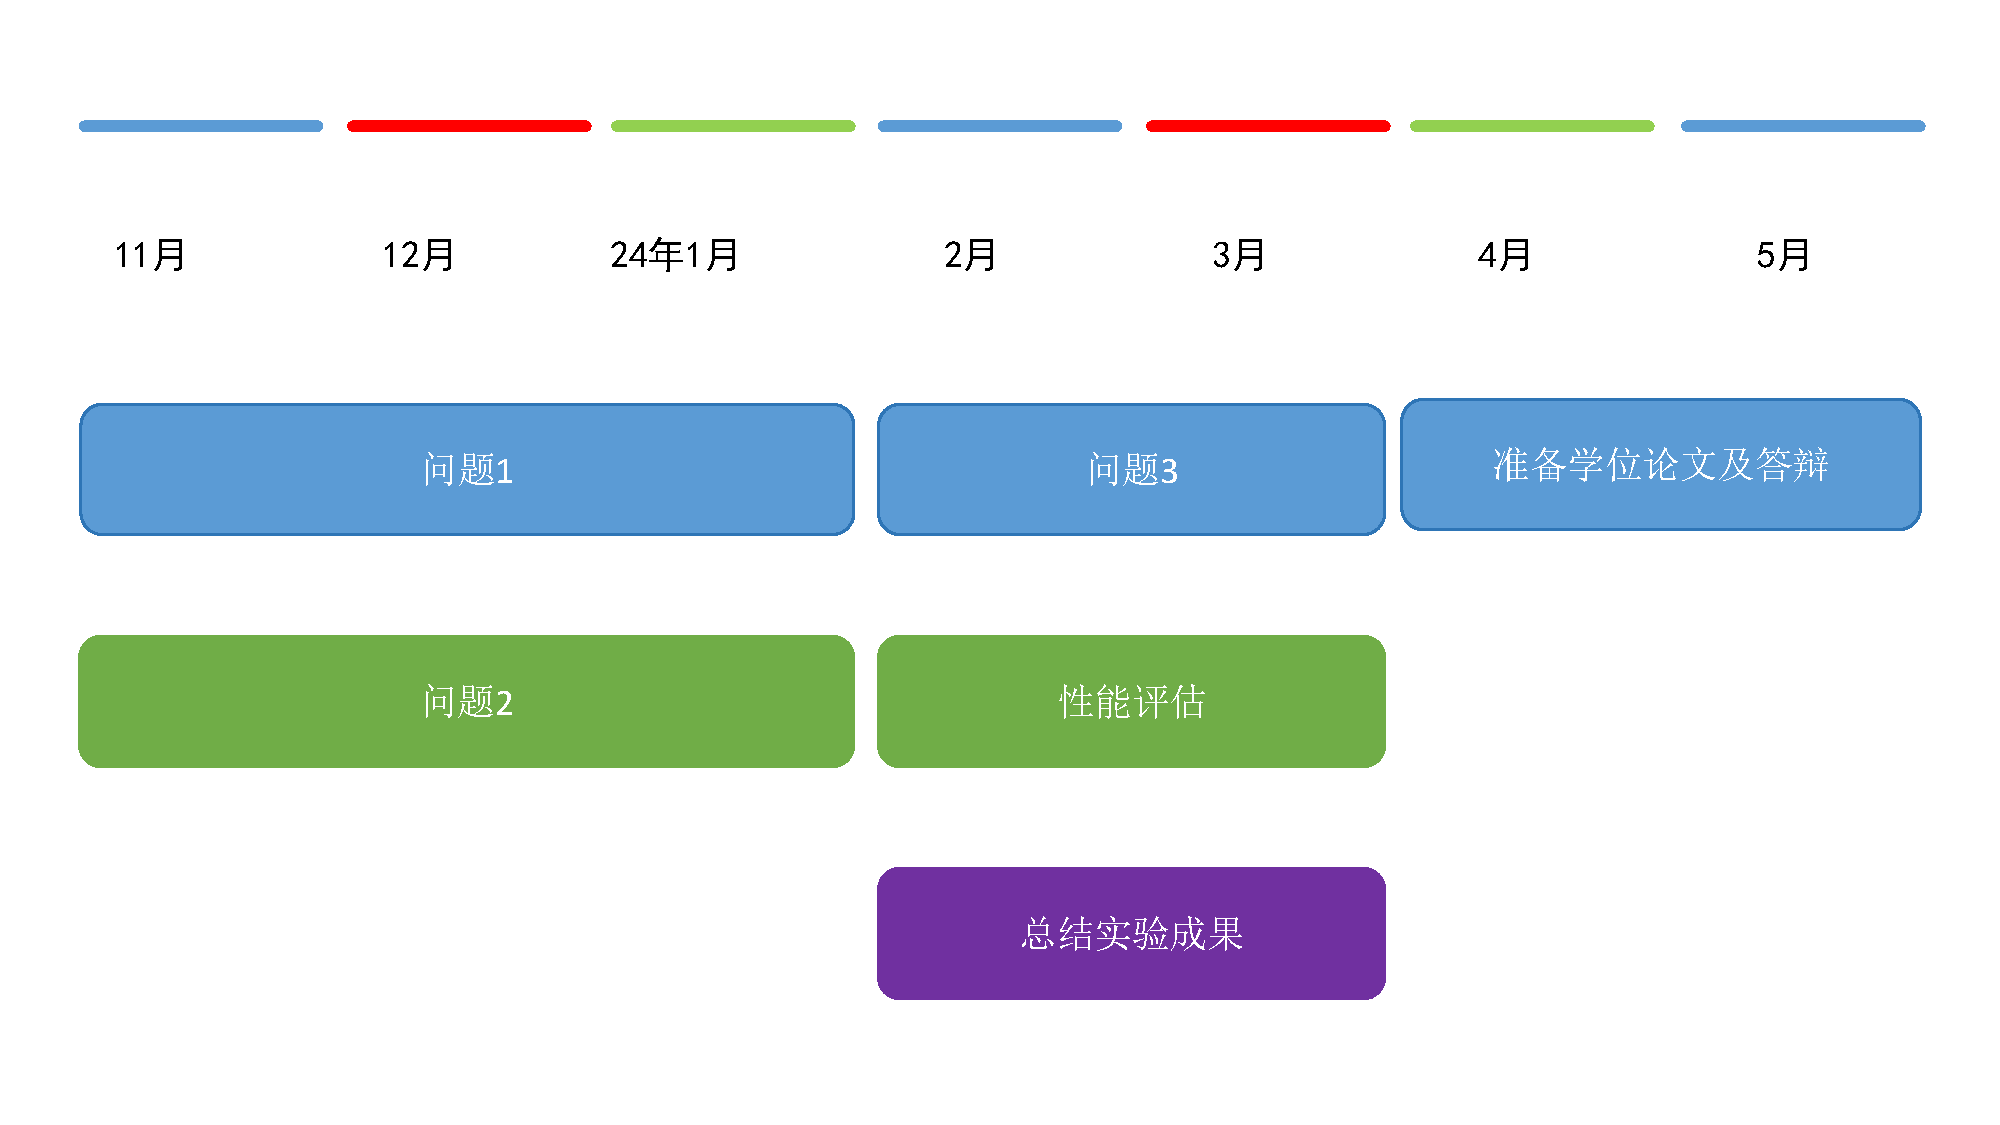
\includegraphics[width=\linewidth]{./images/job_plan.pdf}
  \caption{课题及论文工作计划}
  \label{fig:job_plan}
\end{figure}
 

\clearpage
\bibliography{ref} % 参考文献源,存储所有的参考文献
\bibliographystyle{IEEEtran} % latex饮用参考文献时的格式
\end{document}

